
\clearpage

\subsection{Lubby2: Transient and stationary creep model}
\label{subsec:lubby2}

Viscoplastic creep is mainly caused by diffusion and dislocations at the microscale, and results in hardening as well as recovery aspects. Hou and Lux propose an evolutional equation for the (viscoplastic) creep strain rate considering stationary as well as transient creep, damage impact, hardening and recovery (cf. \cite{Hou:1997,Hou:2002,HL:1998}). Neglecting damage effects, this approach is known as Lubby2 model.
\begin{equation}
\mio{\varepsilon}{\mathrm{c}}{\dot}\,=\,
\frac{3}{2}\,
\left[
\frac{1}{\eta_k}
\left(
1\,-\,
\frac{\varepsilon^{\mathrm{tr}}}{\mathrm{max}\,\varepsilon^{\mathrm{tr}}}
\right)
\,+\,\frac{1}{\eta_m}
\right]
\,\mio{s}{}{}
\label{lubby2_ec}
\end{equation}

Here $\mio{s}{}{}$ denotes the deviatoric stress tensor
\begin{equation}
\mio{s}{}{}\,=\,\mio{\sigma}{}{}\,-\,\frac{1}{3}(\mathrm{tr}\,\mio{\sigma}{}{})\,\mio{I}{}{}
\end{equation}
and $\varepsilon^{\mathrm{tr}}$ the equivalent transient creep strain
\begin{equation}
\varepsilon^{\mathrm{tr}}\,=\,
\sqrt{\frac{2}{3}\,\mio{\varepsilon}{\mathrm{tr}}{}\ccdot\mio{\varepsilon}{\mathrm{tr}}{}}
\end{equation}
with $\mio{\varepsilon}{\mathrm{tr}}{}=\mio{\varepsilon}{\mathrm{c}}{}-\mio{\varepsilon}{\mathrm{st}}{}$ ($\mio{\varepsilon}{\mathrm{st}}{}$ -- stationary creep fraction). In addition to the equivalent transient creep strain the generalized representation of the von~Mises equivalent deviatoric stress $s_{\mathrm{v}}$ is defined.
\begin{equation}
s_{\mathrm{v}}\,=\,\sqrt{\frac{3}{2}\,\mio{s}{}{}\ccdot\mio{s}{}{}}
\end{equation}

Furthermore, the following material functions are suggested, considering only hardening, and neglecting recovery effects:
\begin{eqnarray}
\mathrm{max}\,\varepsilon^{\mathrm{tr}} & \!\!\!\!= &
\!\!\!\!\frac{s_{\mathrm{v}}}{G_k}
\\[2.0ex]
G_k & \!\!\!\!= &
\!\!\!\!{\bar G}^{\ast}_k\,\mathrm{exp}
\left(
k_1\,s_{\mathrm{v}}
\right)\;\,\qquad\qquad\mbox{(Kelvin shear modulus)}
\label{lubby2_f2}
\\[2.0ex]
\eta_k & \!\!\!\!= & \!\!\!\!{\bar\eta}^{\ast}_k\,\mathrm{exp}
\left(
k_2\,s_{\mathrm{v}}
\right)\;\;\,\qquad\qquad\mbox{(Kelvin viscosity modulus)}
\label{lubby2_f3}
\\[2.0ex]
\eta_m & \!\!\!\!= & \!\!\!\!{\bar\eta}^{\ast}_m\,\mathrm{exp}
\left(
m\,s_{\mathrm{v}}
\right)\,\mathrm{exp}(lT)\quad\mbox{(Maxwell viscosity modulus)}
\label{lubby2_f4}
\end{eqnarray}

As $\;T$ denotes the absolute temperature, the following material
parameters are necessary to model various constitutive effects:
\begin{list}{$\bullet$}{\topsep0mm \partopsep0mm \leftmargin6mm
   \parsep0ex \itemsep0.75ex}
\item ${\bar G}^{\ast}_k\,,\;k_1$ \hspace*{3.0ex} hardening,
%\item ${\bar G}^{\ast}_{kE}\,,\;k_{1E}$ \hspace*{0.4ex} recovery,
\item ${\bar\eta}^{\ast}_k\,,\;k_2$ \hspace*{4.0ex} transient creep, and
\item ${\bar\eta}^{\ast}_m\,,\;m\,,\;l$ \hspace*{1.0ex} stationary creep.
\end{list}

\clearpage

\subsubsection*{Problem definition}

Triaxial long-term compression under axisymmetric conditions is carried out to verify the Lubby2 creep model, and to study transient as well as stationary creep behavior assuming isothermal conditions and neglecting damage processes. As described in Sec.~\ref{subsec:lubby1}, for the calculation, the cross-section of a cylindrical sample with a radius of 30~mm and a height of 120~mm is studied. The loading in principal axes includes a radial pressure as well as an axial pressure, and is realized in two steps. It is resulting in a homogeneous stress-strain state. Details of the model (geometry, mesh, boundary conditions) according to K.-H. Lux and F. Werunsky (unpublished report, 2008) are presented in Fig.~\ref{triax_model_lubby2}.

\begin{figure}[!htb]
\begin{center}
\includegraphics[width=0.2\textwidth]{M/figure/svv_model.eps}
\hspace*{10.0ex}
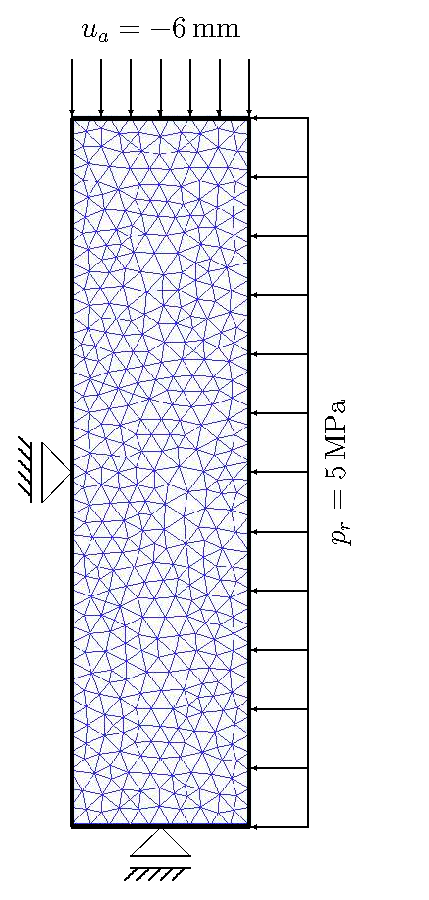
\includegraphics[width=0.25\textwidth]{M/figure/svv_mesh.eps}
\end{center}
\caption{Triaxial compression of a cylindrical sample. Axisymmetric model. Left: Geometry. Right: Finite element grid and boundary conditions.} 
\label{triax_model_lubby2}
\end{figure}

\subsubsection*{Initial and boundary conditions}

Initial conditions do not have to be given for the problem under consideration. As the bottom edge is fixed in vertical direction, the left-hand edge is fixed in horizontal direction for symmetry reasons (axis of rotation). On the right-hand edge initially a radial casing pressure of 5~MPa is applied within 60~seconds with a constant stress rate. While keeping constant this radial pressure, a subsequent stress-driven axial compressive loading is applied within the following 1\,440~seconds with a constant stress rate. The maximum axial pressure is 18~MPa. In the following, both the radial and the axial pressures are kept constant for 20~days (for the loading history cf. Fig.~\ref{triax_loadhist_lubby2}).

\clearpage

\begin{figure}[!htb]
\begin{center}
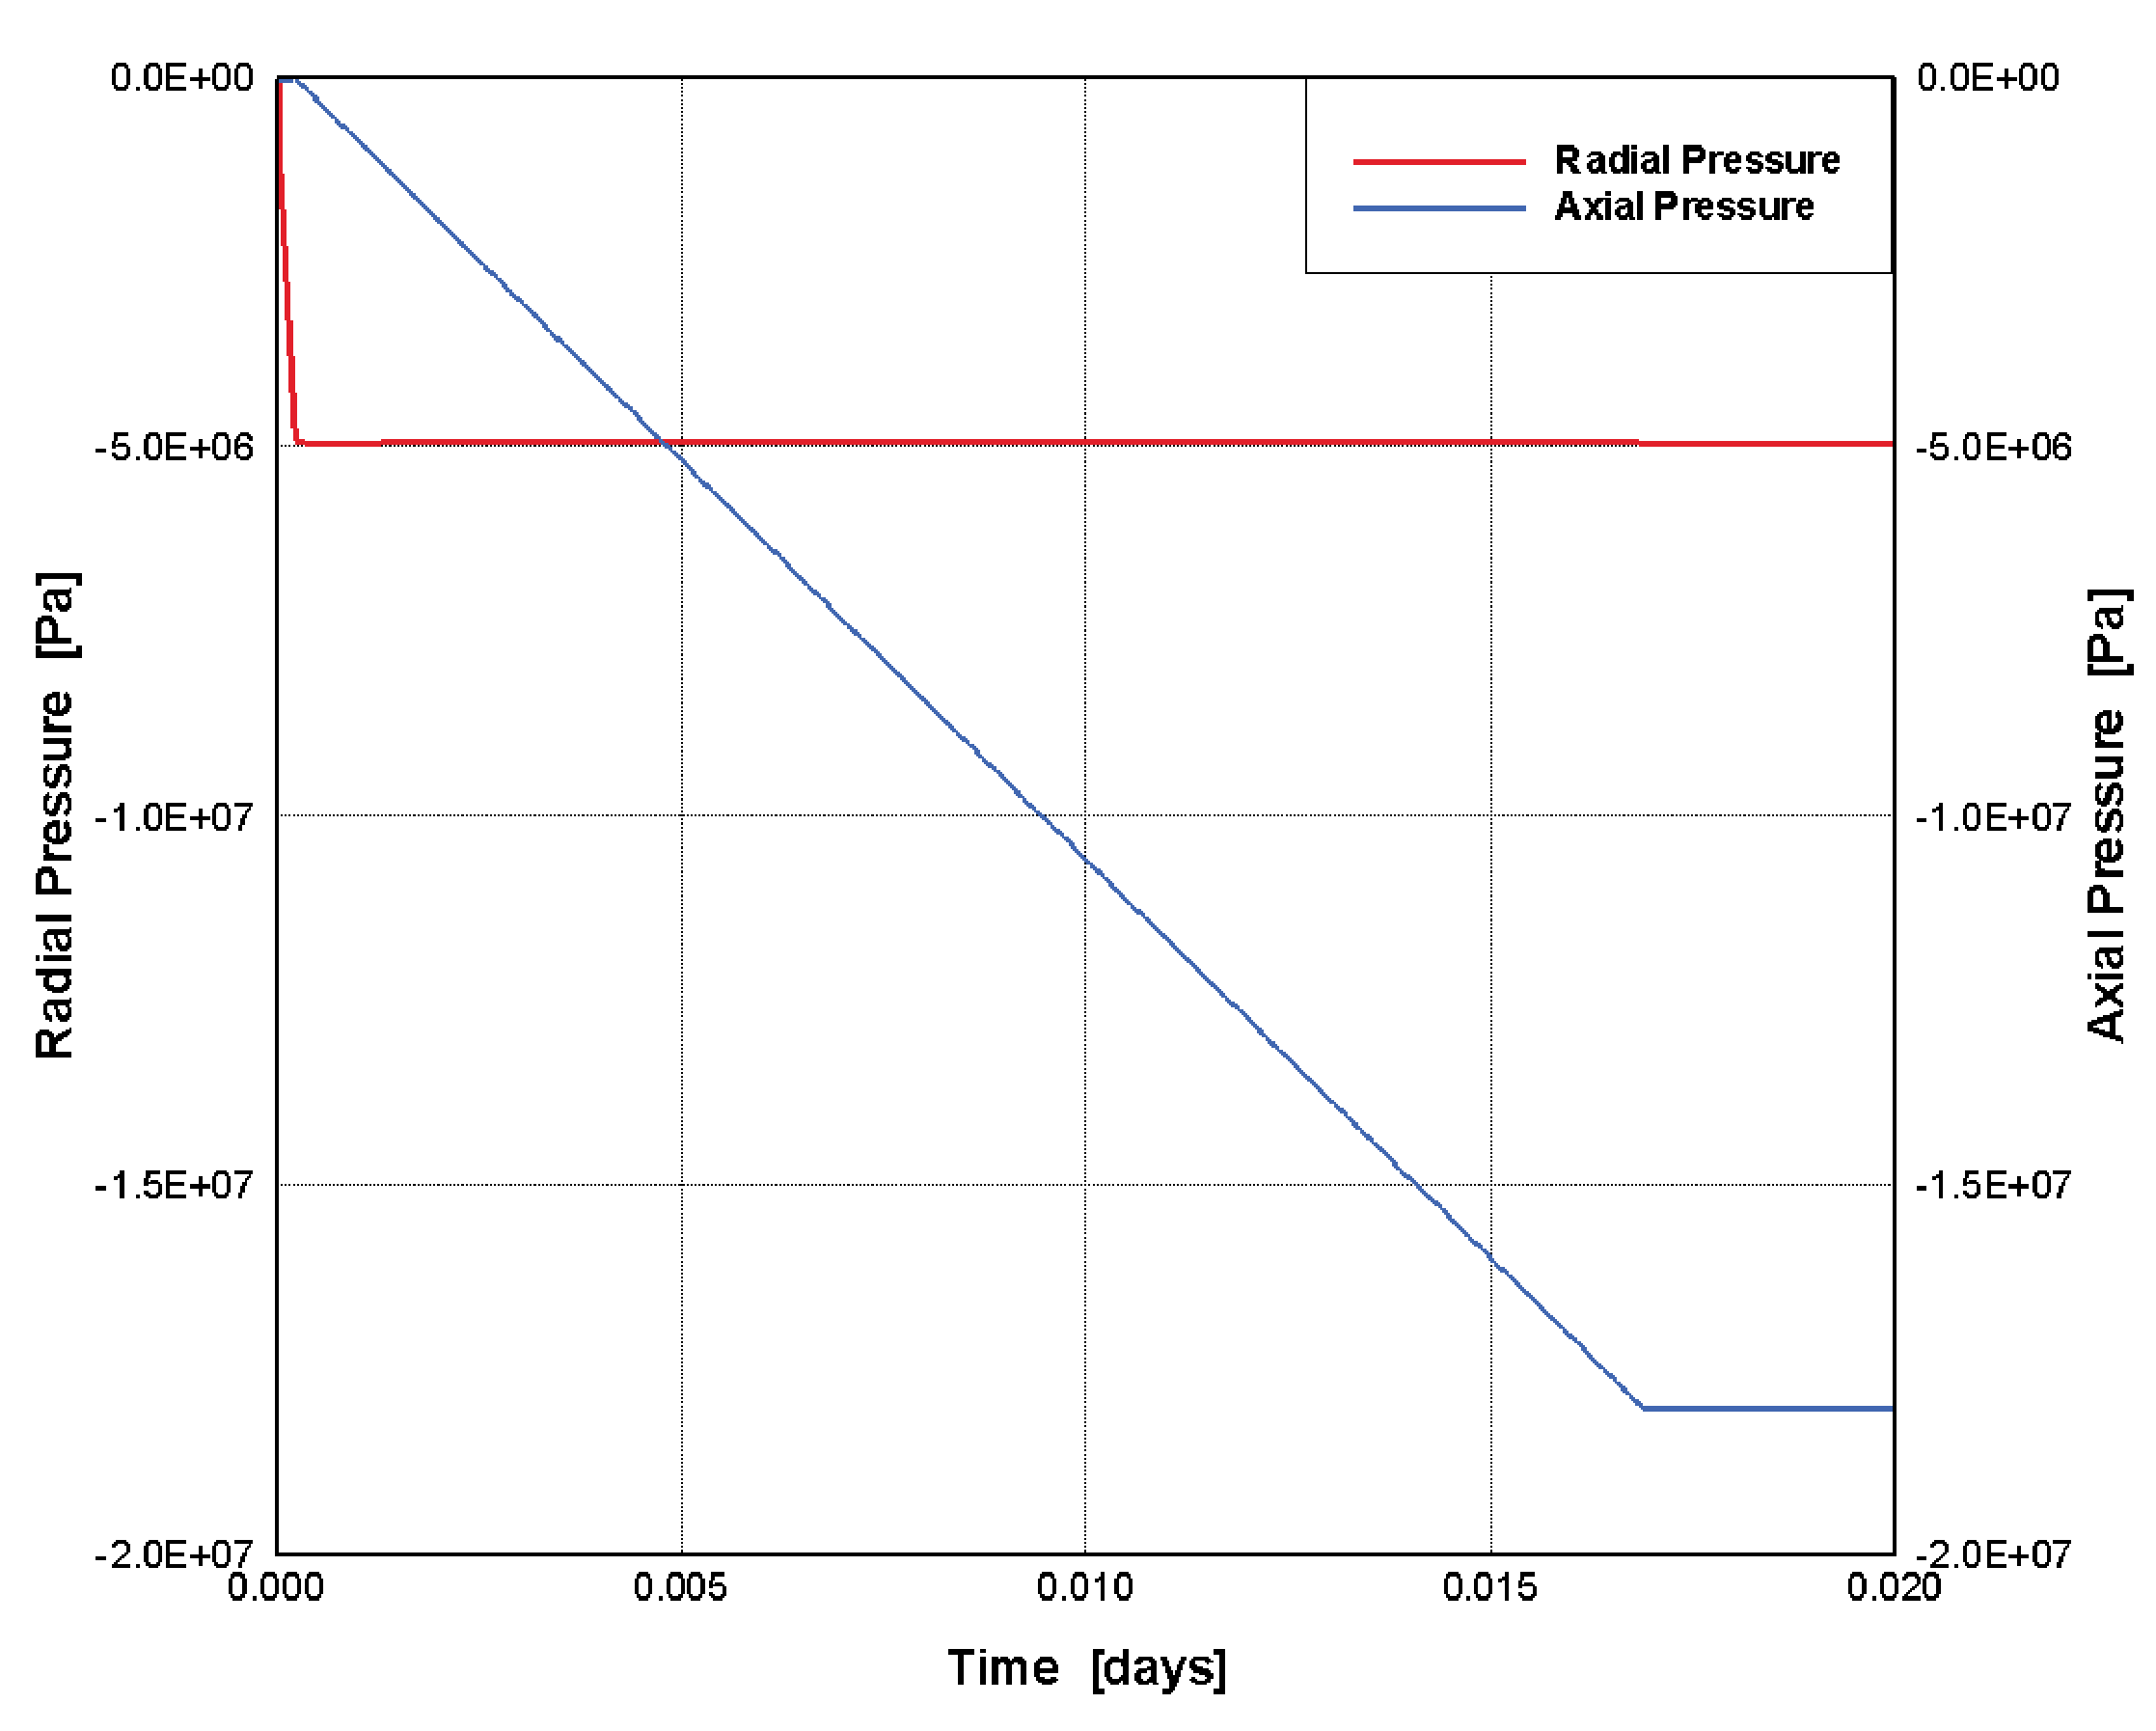
\includegraphics[width=0.6\textwidth]{M/figure/creep/svvcreep_e_HL_loadhistory.eps}
\end{center}
\caption{Triaxial compression of a cylindrical sample. Loading history for long-term creep experiments. Radial casing pressure (stress rate $\dot{p}{}_r=0.083$\,MPa$\cdot$s$^{-1}$) with subsequent axial pressure (stress rate $\dot{p}{}_a=0.0125$\,MPa$\cdot$s$^{-1}$). Each pressure loading with subsequent constant values over 20 days.} 
\label{triax_loadhist_lubby2}
\end{figure}

\subsubsection*{Material properties}

The modified Lubby1 model was considered to generate the fourth-order elastic material matrix for the creep model under consideration. Within this context, the material parameters referring to the modified Lubby1 relation~(\ref{lubby1_ev}) are given in Tab.~\ref{matpar_lubby2_1}. The material parameters for the creep fraction (Lubby2 (\ref{lubby2_ec})) are given in Tab.~\ref{matpar_lubby2_2}. Within this context, the initial Young's modulus, the Poisson's ratio and all the creep parameters are close to values known for rock salt according to K.-H. Lux, M. Rutenberg and F. Werunsky (unpublished report, 2008). 
 
\begin{table}[!htb]
\centering
\begin{tabular}{lll}
\hline\hline\noalign{\smallskip}
Property & Value & Unit \\
\noalign{\smallskip}\hline\noalign{\smallskip}
Poisson's ratio $\nu$             & 0.335   & --  \\
initial Young's modulus $E_0$     & 21\,400 & MPa \\
factor $a$ in (\ref{lubby1_ev})   & 27\,500 & --  \\
exponent $n$ in (\ref{lubby1_ev}) & 1.0     & --  \\
\noalign{\smallskip}\hline\hline
\end{tabular}
\caption{Material parameters for the elastic fraction of the material model (cf.~Sec.~\ref{subsec:lubby1})}
\label{matpar_lubby2_1}
\end{table}
 
\begin{table}[!htb]
\centering
\begin{tabular}{lll}
\hline\hline\noalign{\smallskip}
Property & Value & Unit \\
\noalign{\smallskip}\hline\noalign{\smallskip}
Maxwell viscosity ${\bar\eta}^{\ast}_m$ in (\ref{lubby2_f4})  & $1.09\cdot 10^7$ & MPa$\cdot$day \\
factor $m$ in (\ref{lubby2_f4})                               & $-0.219$         & MPa$^{-1}$    \\
factor $l$ in (\ref{lubby2_f4})                               & $0.0$            & K$^{-1}$      \\
Kelvin viscosity ${\bar\eta}^{\ast}_k$ in (\ref{lubby2_f3})   & $1.45\cdot 10^5$ & MPa$\cdot$day \\
factor $k_1$ in (\ref{lubby2_f2})                             & $-0.146$         & MPa$^{-1}$    \\
factor $k_2$ in (\ref{lubby2_f3})                             & $-0.121$         & MPa$^{-1}$    \\
Kelvin shear modulus ${\bar G}^{\ast}_k$ in (\ref{lubby2_f2}) & $7.0\cdot 10^4$  & MPa           \\
\noalign{\smallskip}\hline\hline
\end{tabular}
\caption{Material parameters for the creep fraction of the material model}
\label{matpar_lubby2_2}
\end{table}


\subsubsection*{Results}

The representation of the axial stress vs. the axial strain in Fig.~\ref{triax_res_lubby2} shows the complex creep behavior of the sample under consideration.

\begin{figure}[!htb]
\begin{center}
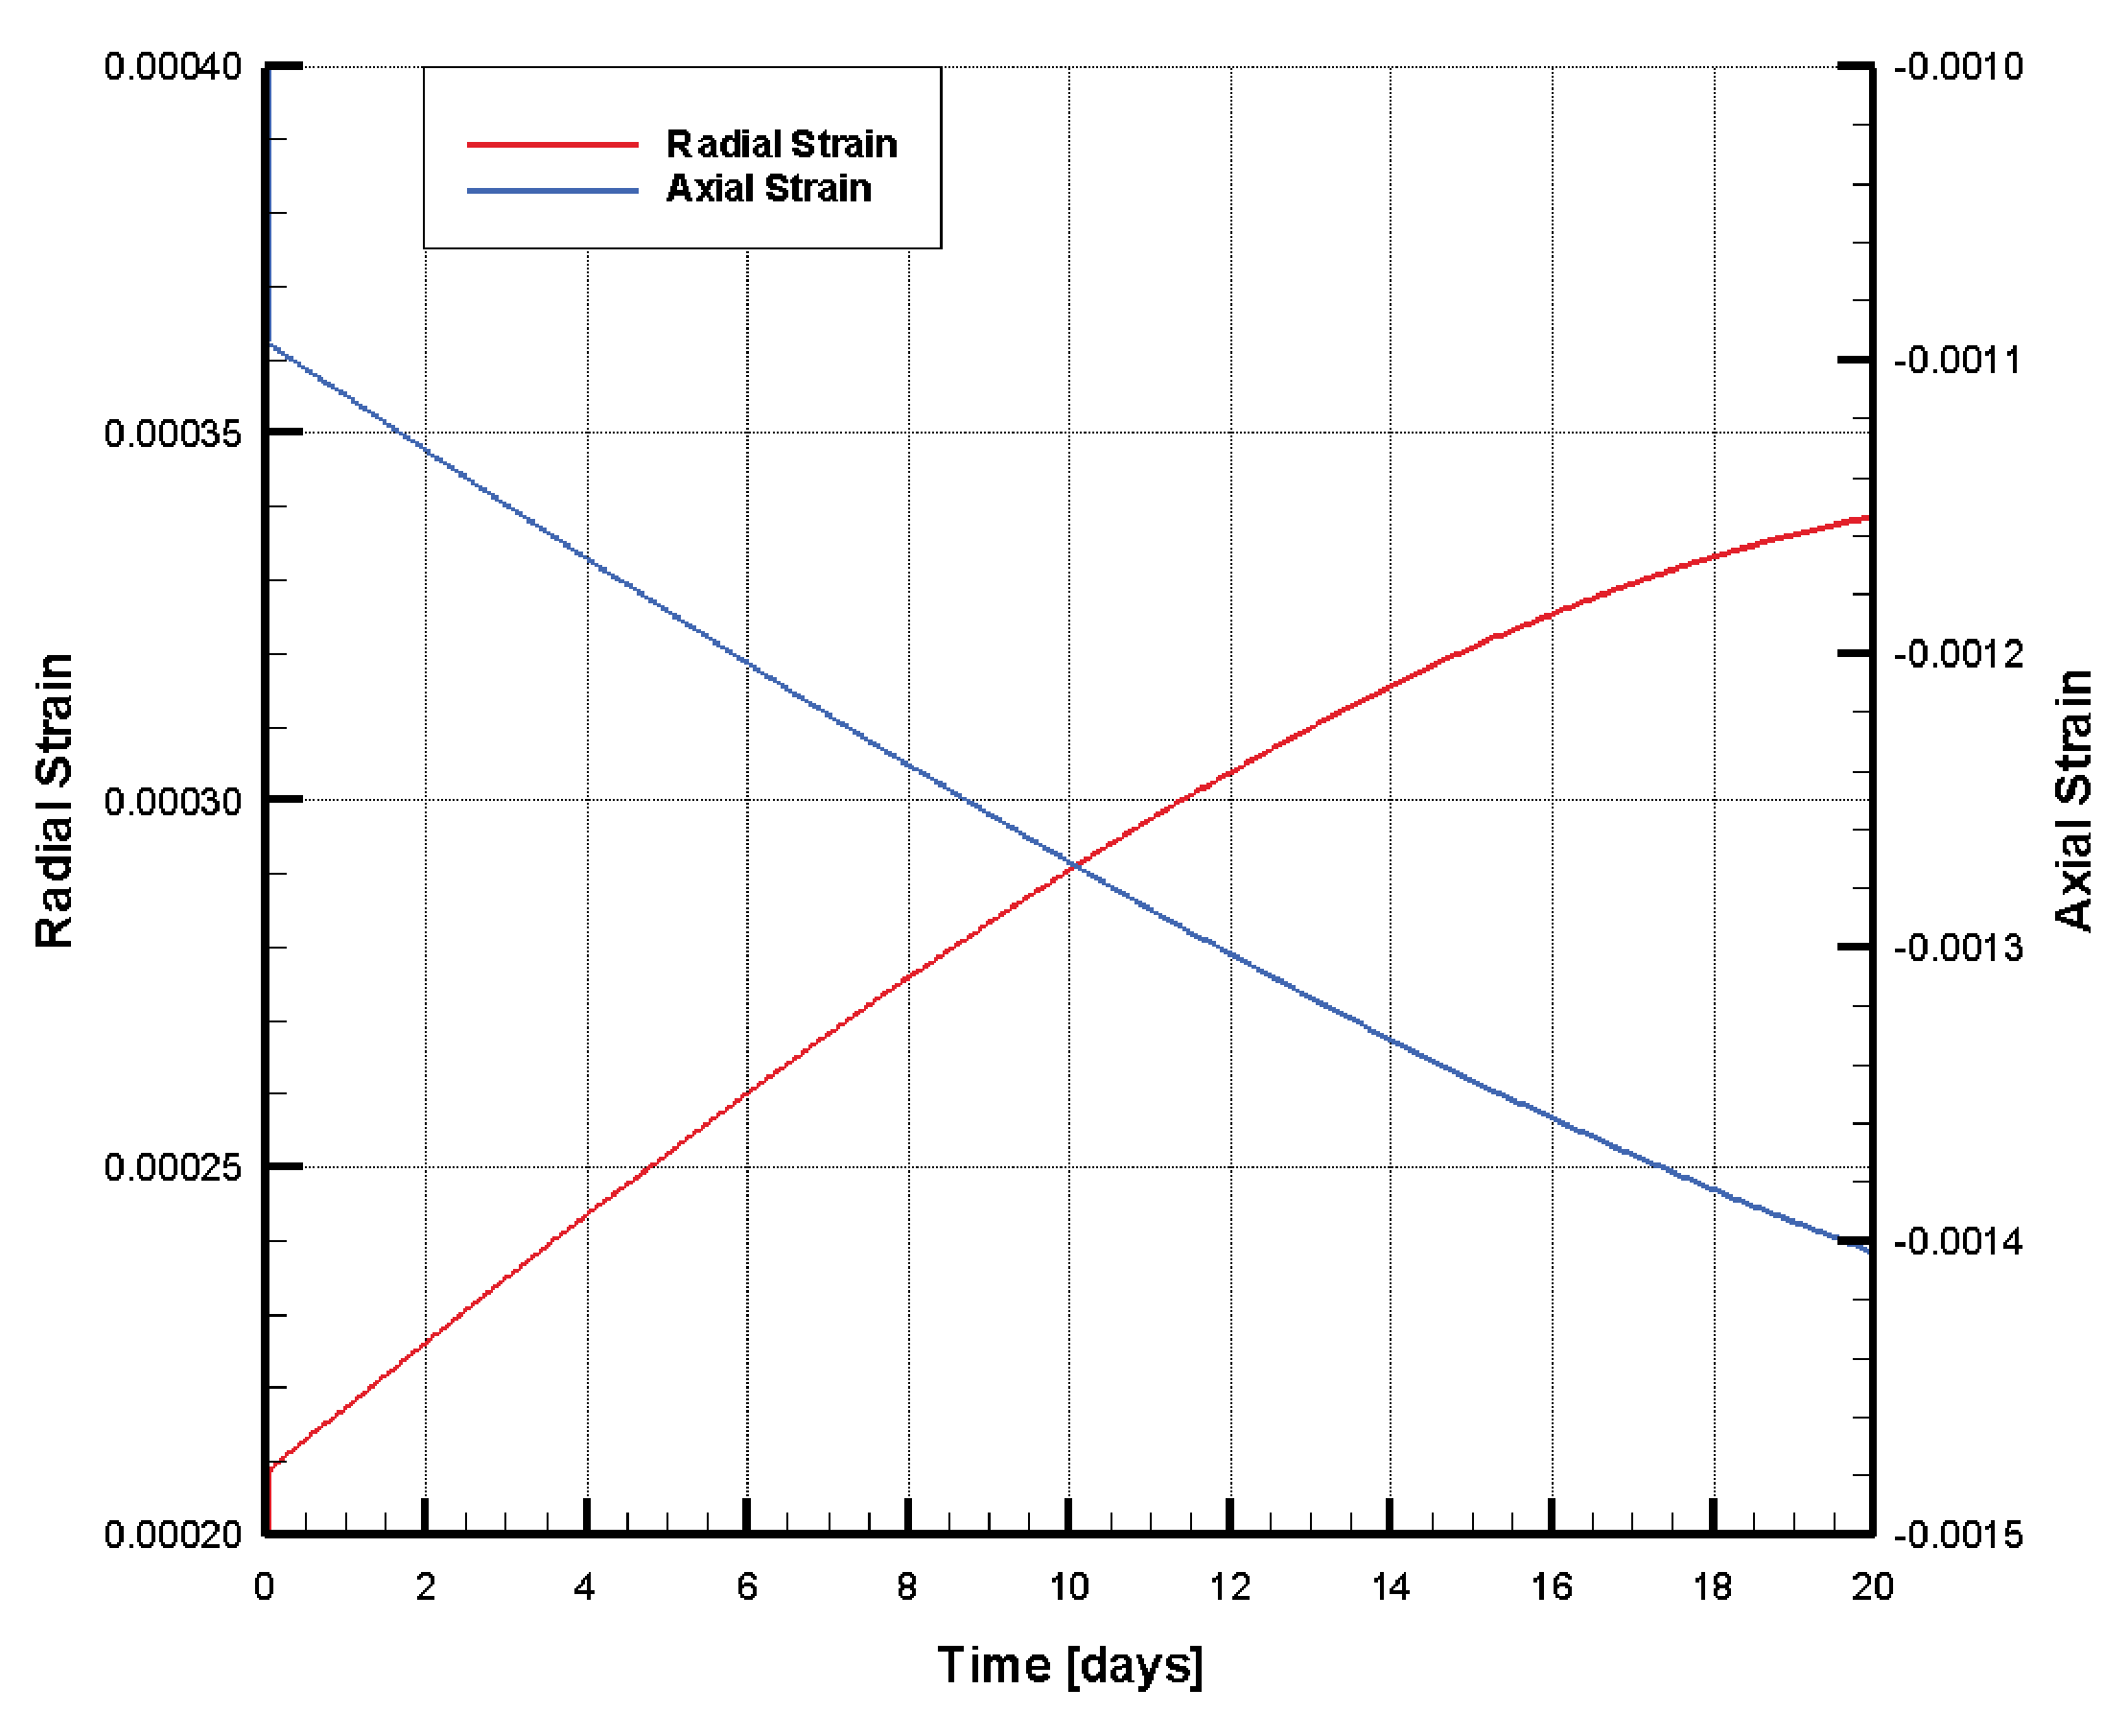
\includegraphics[width=0.6\textwidth]{M/figure/creep/svvcreep_e_HL_strain.eps}
\end{center}
\caption{Triaxial compression of a cylindrical sample. Numerical simulation of the transient and stationary creep behavior using the Lubby2 model~(\ref{lubby2_ec}).} 
\label{triax_res_lubby2}
\end{figure}

\subsubsection*{Benchmark deposit}

\begin{tabular}{|l|l|l|}
  \hline
  Benchmark & Problem type & Path in benchmark deposit \\
  \hline
 \emph{m\_triax\_lubby2} & M & benchmarks\verb \M\creep \\
  \hline
\end{tabular}
